\section{Introduction}
\label{sec:intro}

Mixture-of-Experts (MoE) architectures have emerged as a prominent approach for scaling Large Language Models (LLMs) to hundreds of billions of parameters~\cite{shazeer2017outrageously,fedus2022switch, jiang2024mixtral,dai2024deepseekmoe}. 
By dynamically routing each token to only a sparse subset of experts, MoE models substantially increase model capacity while keeping per-token computation bounded~\cite{du2022glam,rajbhandari2022deepspeedmoe}. 
However, sparse activation reduces computation rather than model storage: although only a small number of experts are activated for each token, the runtime must still make the entire expert pool available for routing. 
As MoE models scale, the simultaneous residency of all expert weights in accelerator High-Bandwidth Memory (HBM) places significant strain on memory capacity.
To serve such models on memory-constrained accelerators, \textbf{expert offloading} has become an important strategy: the runtime keeps non-expert layers and a bounded subset of frequently used experts in local HBM, while fetching non-resident experts from host memory on demand~\cite{hwang2024pregated,xue2024moeinfinity,li2026commitmoe}. 

To make expert offloading practical, prior systems reduce its data-movement overhead through expert caching, routing-aware prediction and prefetching, and transfer--computation overlap~\cite{hwang2024pregated,kong2024swapmoe,cao2025moelightning,fang2025klotski,xue2024moeinfinity}. 
These techniques reduce the frequency of host-to-device transfers or hide part of their latency, substantially improving the efficiency of offloaded MoE inference. 
However, they do not eliminate the inherent execution dynamism introduced by expert offloading. 
Loading and replacing experts in a bounded HBM cache can change the mapping between logical experts and their physical weight locations across decoding steps. 
Thus, existing data-movement optimizations improve which experts are moved and when they are moved, but they do not eliminate runtime changes in logical-to-physical weight bindings. 

Such runtime changes can be naturally accommodated under eager execution, where the host resolves the current expert placement and dispatches the corresponding kernels at each decoding step. This flexibility, however, comes at a substantial performance cost. Autoregressive decoding repeatedly executes a largely recurring sequence of fine-grained accelerator kernels, and launching these kernels individually incurs repeated host-side scheduling, dispatch, and synchronization overhead. \textbf{Graph replay} mitigates this overhead by capturing the recurring execution sequence once and replaying it as a unit, thereby reducing host-induced gaps between kernel executions~\cite{kwon2020nimble,ye2025flashinfer}. 

As shown in Figure~\ref{fig:graph_breakdown}, graph replay reduces average decode latency by approximately 75\% across four workloads, from 133.7--137.4~ms/token under eager execution to 32.6--33.6~ms/token, while device execution time remains nearly unchanged. 
This result indicates that most of the improvement comes from eliminating host-induced device idle time rather than accelerating the underlying kernels. 

\begin{figure}[t] 
  \centering 
  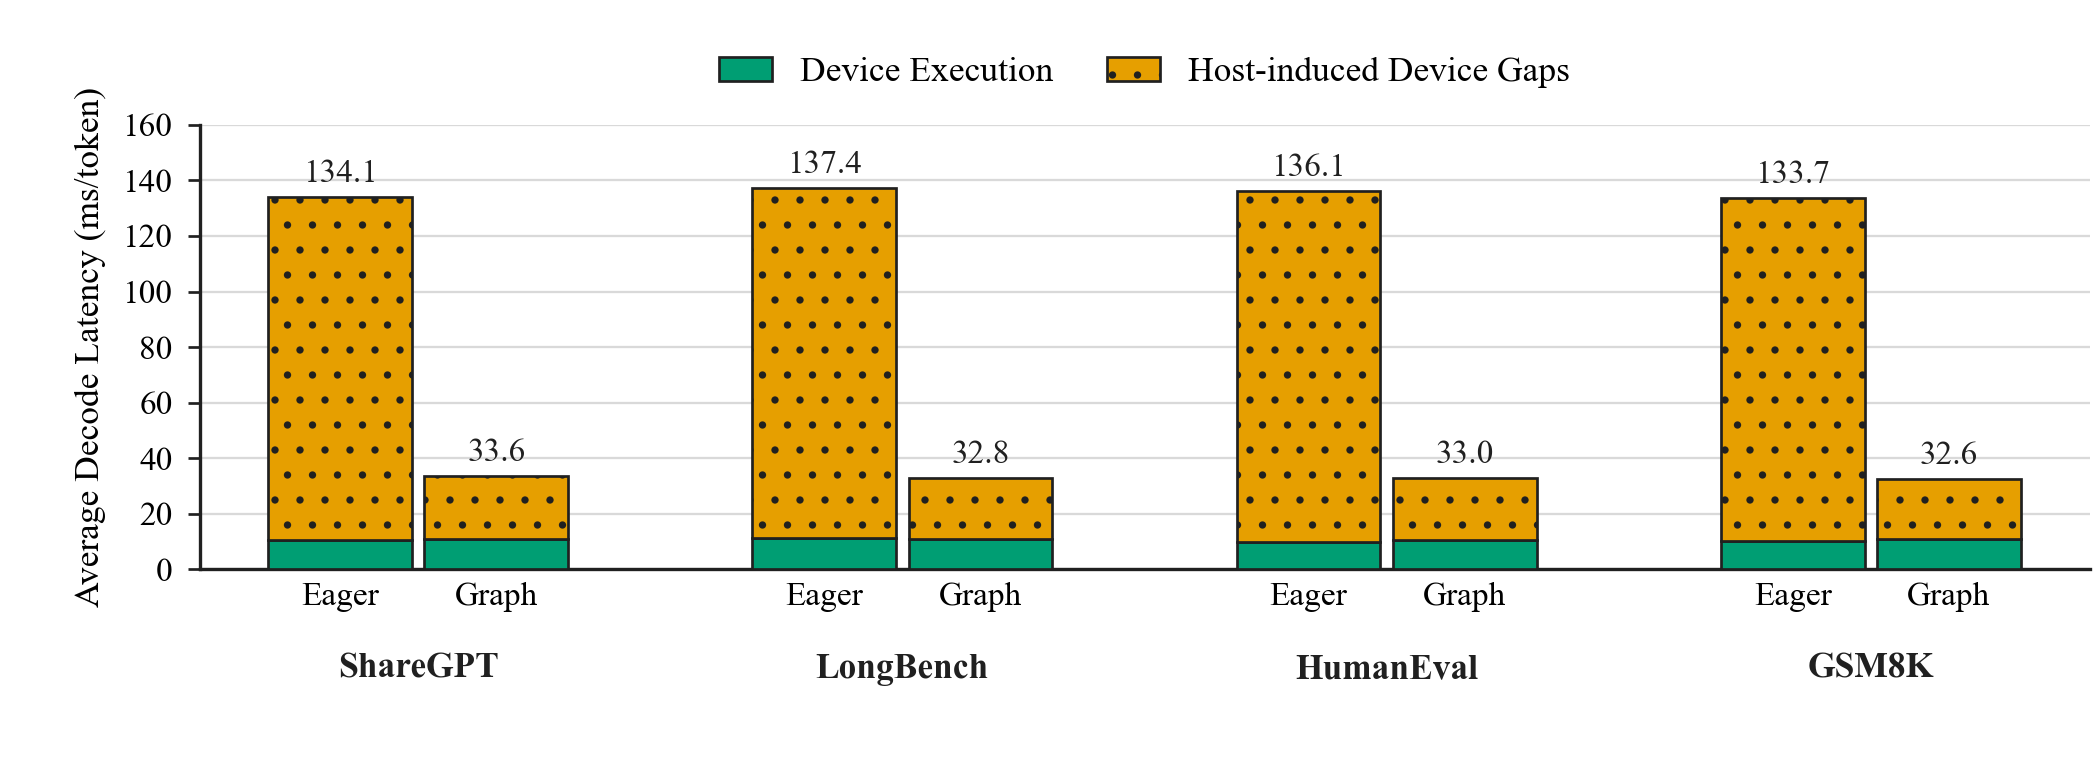
\includegraphics[width=1\linewidth]{figures/graph_breakdown.png} 
  \caption{Average decode latency breakdown under eager execution and graph replay. Graph replay substantially reduces host-induced device gaps while leaving device execution time nearly unchanged.} 
  \label{fig:graph_breakdown} 
\end{figure} 

However, graph replay is effective only when the captured execution state, including its memory bindings, remains stable. 
Dynamic expert offloading can violate this condition. 
A cache miss may trigger expert eviction and replacement, causing the logical-to-physical weight binding to change across decoding steps.
The captured computation then cannot safely reuse its previous bindings without repairing the graph or falling back to eager execution. 
Both options add host work and reduce the benefit of graph replay. 
The resulting systems problem is to \textbf{enable dynamic expert residency and placement without sacrificing graph replay under a bounded HBM budget }.

Graph-compatible inference runtimes take a different approach: they keep graph-visible workspaces, metadata, and execution configurations reusable across replays~\cite{ye2025flashinfer}. However, they do not support a bounded expert pool whose contents change dynamically. Therefore, existing systems lack an execution abstraction that supports dynamic expert replacement while preserving graph replay.

Our key insight is that \textbf{graph replay requires stable physical storage, not static expert residency}. Captured computation only requires its graph-visible storage addresses to remain valid. The runtime can therefore reuse a fixed set of physical slots for different logical experts: replacement changes slot contents and mapping values, not the addresses visible to the graph. This separation allows expert residency to evolve under a bounded HBM budget without invalidating replay.

Realizing this abstraction raises three systems challenges.
First, routing-dependent expert staging must occur without invalidating captured computation.
Active experts are known only after routing, yet loading and replacement must not alter the replay-visible storage or execution structure.
Second, bounded slot storage must be updated without placing expert transfer entirely on the critical path.
Changing routing decisions may require repeated expert movement, and the routed working set may exceed the available slots, making transfer--computation overlap essential for efficient execution.
Third, slot reuse must remain correct under asynchronous transfer and computation.
A slot cannot be reassigned while its previous contents are still in use, nor can a new assignment become visible before the staged weights are ready.

We present \system, a graph-compatible MoE offloading system that virtualizes dynamic logical experts over a fixed physical slot interface.
To isolate routing-dependent dynamism from captured computation, \system places expert staging at an eager boundary while keeping the physical storage seen by replayed kernels stable.
It further pipelines expert staging and computation through wave-based execution, allowing bounded slot storage to be reused while overlapping transfers for upcoming experts with ongoing computation.
Finally, a version-controlled handoff protocol coordinates transfer readiness,computation, and mapping publication to ensure safe slot reuse.
Together, these mechanisms preserve replay-stable execution while allowing expert residency and placement to evolve dynamically under constrained HBM.

In summary, this paper makes the following contributions:

\begin{itemize}

\item We identify a cross-layer conflict between dynamic expert offloading and graph replay in memory-constrained MoE inference: routing-driven expert replacement changes logical-to-physical weight bindings, whereas graph replay depends on a stable graph-visible execution state. 
From this conflict, we derive the key insight that replayability requires stable physical storage rather than static expert residency.

\item We design \system, a graph-compatible MoE offloading runtime that virtualizes dynamic logical experts over replay-stable physical slots.
\system isolates routing-dependent expert staging from captured computation, pipelines expert transfer with computation through wave-based execution, and coordinates safe slot reuse through a version-controlled handoff protocol.

\item We implement \system on top of vLLM-Ascend and evaluate it under constrained HBM. 
On Qwen3-30B-A3B, \system preserves exact model outputs and graph replay under dynamic expert offloading. Compared with graph-compatible full-layer staging, its multi-wave prefill execution reduces repeat-median TTFT p50 by 35.21\%.

\end{itemize}
